\documentclass[11pt]{article}

% ====================================================
% ====================================================
% USEPACKAGES AND IMPORTS
% ====================================================
% ====================================================

\usepackage[T1]{fontenc}
\usepackage[utf8]{inputenc}
\usepackage[english]{babel}

\usepackage{fancyhdr}

% definitions
% ====================================================
\let\titleoriginal\title
\renewcommand{\title}[1]{
	\titleoriginal{#1}
	\newcommand{\thetitle}{#1}
}

\setlength{\parskip}{\baselineskip}%
\setlength{\parindent}{0pt}%

% header and footer
\pagestyle{fancy}
\fancyhf{}
\lhead{Applied Machine Learning Fundamentals}
\rhead{\thetitle}
\cfoot{\thepage}

% ====================================================
% ====================================================
% BEGIN OF DOCUMENT
% ====================================================
% ====================================================
\begin{document}

\mytitle{Exercise 4 - Backpropagation and unsupervised Learning}
\myauthor{student1, student2, student3}
\firstpage{\insertmytitle}{Winter term 2019/2020}{\insertmyauthor}

% Backprop
%______________________________________________________________________
\section{Backpropagation}

\begin{enumerate}[label=\alph*)]

% Task 1
\exercise{Backpropagation by Hand (5 points)}{
You are given the neural network depicted below. Compute one forward-pass and one backward-pass based on the labeled training example $\langle \bm{x} = [0.05, 0.10], \bm{y} = [0, 1] \rangle$. 
Employ the squared error loss function:

\begin{align*}
	\mathcal{J}(\bm{\Theta})
		&= (y_{pred} - y)^2 \\[3mm]
	\mathcal{J}'(\bm{\Theta})
		&= 2 \cdot (y_{pred} - y)
\end{align*}

The weight matrices and bias weights are initialized as follows (where for instance weight $\Theta_{12}^{(1)}$ connects the input $x_2$ with the first neuron in the hidden layer):

\begin{minipage}{0.49\textwidth}
	\begin{align*}
		\bm{\Theta}^{(1)}
			&= \begin{pmatrix}
				0.15 & 0.20 \\
				0.25 & 0.30
			\end{pmatrix} \\[3mm]
		\bm{b}^{(1)}
			&= \begin{pmatrix}0.35 & 0.35\end{pmatrix}
	\end{align*}
\end{minipage}
\hfill
\begin{minipage}{0.49\textwidth}
	\begin{align*}
		\bm{\Theta}^{(2)}
			&= \begin{pmatrix}
				0.40 & 0.45 \\
				0.50 & 0.55
			\end{pmatrix} \\[3mm]
		\bm{b}^{(2)}
			&= \begin{pmatrix}0.60 & 0.60\end{pmatrix}
	\end{align*}
\end{minipage}
\vspace*{5mm}

Use the ReLU and sigmoid activation functions in the hidden layer and output layer, respectively. Write down all necessary computations.
What are the gradients for the weights $\Theta_{12}^{(1)}$, $\Theta_{21}^{(2)}$?
\begin{figure}[h]
	\centering
	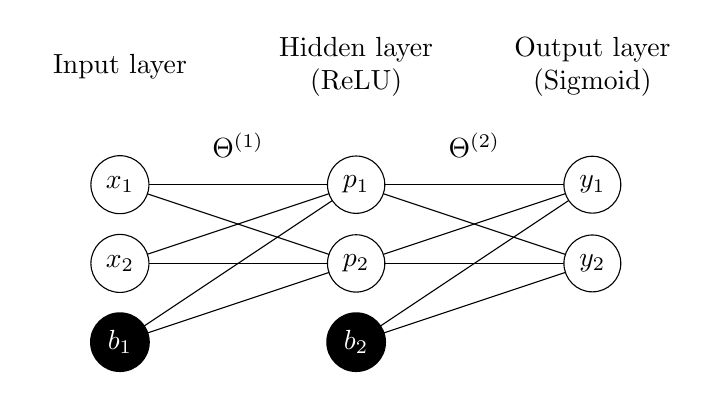
\begin{tikzpicture}[
		neuron/.style={circle,minimum size=17pt,fill=white,draw=black},
		bias/.style={circle,minimum size=17pt,fill=black},
		annot/.style={text width=6em, text centered}
	]

		% connect input and hidden layers
		\foreach \i in {0,1,2}
		    \foreach \h in {1,2}
		            \draw[-stealth] (0,\i) -- (3,\h);
		
		% connect hidden and output layers
		\foreach \h in {0,1,2}
			\foreach \o in {1,2}
				\draw (3,\h) -- (6,\o);
				
		\node[neuron] at (0,2) {$x_1$};
		\node[neuron] at (0,1) {$x_2$};
		\node[bias] at (0,0) {\textcolor{white}{$b_1$}};

		\node[neuron] at (3,2) {$p_1$};
		\node[neuron] at (3,1) {$p_2$};
		\node[bias] at (3,0) {\textcolor{white}{$b_2$}};

		\node[neuron] at (6,2) {$y_1$};
		\node[neuron] at (6,1) {$y_2$};
		            
		% annotate the layers
		\node[annot] at (0,3.5) {Input layer};
		\node[annot] at (3,3.5) {Hidden layer (ReLU)};
		\node[annot] at (6,3.5) {Output layer (Sigmoid)};
		\node[annot] at (1.5,2.5) {$\bm{\Theta}^{(1)}$};
		\node[annot] at (4.5,2.5) {$\bm{\Theta}^{(2)}$};

	\end{tikzpicture}
	\caption{MLP architecture}
\end{figure}
}{
% >>>> your answer here <<<<
}

\end{enumerate}

\newpage



% Clustering
%______________________________________________________________________
\section{Unsupervised Learning}

\begin{enumerate}[label=\alph*)]

% Task 2
\exercise{$k$-Means clustering (4 points)}{
Implement $k$-Means clustering for image compression. Compress the exemplary image file which can be found under the path \cb{\texttt{/data/dhbw.jpg}}.
You can find an explanation of how image compression with $k$-Means works on this web page.\footnote{\url{https://medium.com/@agarwalvibhor84/image-compression-using-k-means-clustering-8c0ec055103f}}
}{
% >>>> your answer here <<<<
\vspace*{7cm}
}




% Task 3
\exercise{PCA (1 point)}{
Explain how to choose the number of principal components for dimensionality reduction. Why does this work?
}{
% >>>> your answer here <<<<
}

\newpage


% Task 4
\exercise{Bonus Question: Spectral clustering (1 point)}{
How can you automatically choose the number of clusters for spectral clustering?
}{
% >>>> your answer here <<<<
}

\end{enumerate}

\end{document}